
%%%%%%%%%%%%%%%%%%%%%%%%%%%%%%%%%%%%%%%%%%%%%%%%%%%%%%%%%%%%%%%%%%%%%%%%%%%%%%%%%%%%%%%
%%%%%%%%%%%%%%%%%%%%%%%%%%%%%%%%%%%%%%%%%%%%%%%%%%%%%%%%%%%%%%%%%%%%%%%%%%%%%%%%%%%%%%%
% 
% This top part of the document is called the 'preamble'.  Modify it with caution!
%
% The real document starts below where it says 'The main document starts here'.

\documentclass[12pt]{article}

\usepackage{amssymb,amsmath,amsthm}
\usepackage[top=1in, bottom=1in, left=1.25in, right=1.25in]{geometry}
\usepackage{fancyhdr}
\usepackage{enumerate}
\usepackage{listings}
\usepackage{graphicx}
\usepackage{float}
\usepackage{multicol}
% Comment the following line to use TeX's default font of Computer Modern.
\usepackage{times,txfonts}
\usepackage{mwe}
\usepackage{caption}
\usepackage{subcaption}

\usepackage{tikz}
\def\checkmark{\tikz\fill[scale=0.4](0,.35) -- (.25,0) -- (1,.7) -- (.25,.15) -- cycle;} 



\makeatletter
\renewcommand*\env@matrix[1][*\c@MaxMatrixCols c]{%
  \hskip -\arraycolsep
  \let\@ifnextchar\new@ifnextchar
  \array{#1}}
\makeatother

\newtheoremstyle{homework}% name of the style to be used
  {18pt}% measure of space to leave above the theorem. E.g.: 3pt
  {12pt}% measure of space to leave below the theorem. E.g.: 3pt
  {}% name of font to use in the body of the theorem
  {}% measure of space to indent
  {\bfseries}% name of head font
  {:}% punctuation between head and body
  {2ex}% space after theorem head; " " = normal interword space
  {}% Manually specify head
\theoremstyle{homework} 

% Set up an Exercise environment and a Solution label.
\newtheorem*{exercisecore}{Exercise \@currentlabel}
\newenvironment{exercise}[1]
{\def\@currentlabel{#1}\exercisecore}
{\endexercisecore}

\newcommand{\localhead}[1]{\par\smallskip\noindent\textbf{#1}\nobreak\\}%
\newcommand\solution{\localhead{Solution:}}

%%%%%%%%%%%%%%%%%%%%%%%%%%%%%%%%%%%%%%%%%%%%%%%%%%%%%%%%%%%%%%%%%%%%%%%%
%
% Stuff for getting the name/document date/title across the header
\makeatletter
\RequirePackage{fancyhdr}
\pagestyle{fancy}
\fancyfoot[C]{\ifnum \value{page} > 1\relax\thepage\fi}
\fancyhead[L]{\ifx\@doclabel\@empty\else\@doclabel\fi}
\fancyhead[C]{\ifx\@docdate\@empty\else\@docdate\fi}
\fancyhead[R]{\ifx\@docauthor\@empty\else\@docauthor\fi}
\headheight 15pt

\def\doclabel#1{\gdef\@doclabel{#1}}
\doclabel{Use {\tt\textbackslash doclabel\{MY LABEL\}}.}
\def\docdate#1{\gdef\@docdate{#1}}
\docdate{Use {\tt\textbackslash docdate\{MY DATE\}}.}
\def\docauthor#1{\gdef\@docauthor{#1}}
\docauthor{Use {\tt\textbackslash docauthor\{MY NAME\}}.}
\makeatother

% Shortcuts for blackboard bold number sets (reals, integers, etc.)
\newcommand{\Reals}{\ensuremath{\mathbb R}}
\newcommand{\Nats}{\ensuremath{\mathbb N}}
\newcommand{\Ints}{\ensuremath{\mathbb Z}}
\newcommand{\Rats}{\ensuremath{\mathbb Q}}
\newcommand{\Cplx}{\ensuremath{\mathbb C}}
%% Some equivalents that some people may prefer.
\let\RR\Reals
\let\NN\Nats
\let\II\Ints
\let\CC\Cplx

%\textbf{Code:}
%\begin{center}
%  \lstinputlisting{NewtonsMethodP5.m}
%\end{center}
%
%\textbf{Console:}
%\begin{center}
%  \lstinputlisting{P5C.txt}
%\end{center}
%\vspace{.15in}


%\begin{figure}[H]
%  \begin{center}
%    \caption{The one-norm unit ball}
%    \includegraphics[width=.76\textwidth]{1norm.png}
%  \end{center}
%\end{figure}




%%%%%%%%%%%%%%%%%%%%%%%%%%%%%%%%%%%%%%%%%%%%%%%%%%%%%%%%%%%%%%%%%%%%%%%%%%%%%%%%%%%%%%%
%%%%%%%%%%%%%%%%%%%%%%%%%%%%%%%%%%%%%%%%%%%%%%%%%%%%%%%%%%%%%%%%%%%%%%%%%%%%%%%%%%%%%%%
% 
% The main document start here.

% The following commands set up the material that appears in the header.
\doclabel{Math 661: Homework 4}
\docauthor{Stefano Fochesatto}
\docdate{\today}


\begin{document}

\begin{exercise}{2.2} Let $Z$ be an $n x r$ null-space matrix for the matrix $A$. If $Y$ 
  is any invertible $rxr$ matrix, prove that $\hat{Z} = ZY$ is also a null space matrix for $A$.
  \begin{proof} Suppose $Z$ is an $n x r$ null-space matrix for the matrix $A$ and let $Y$ ne 
    an invertible $r x r$ matrix. Consider the matrix $ZY$ and note that since $Y$ is invertible, it's columns 
    form a basis in $R^r$, thus for every $x \in \RR^r$ we know that there exists a $y \in \RR^r$ of the form 
    $y = Y^{-1}x$. Therefore by substitution we know $ZYy = ZYY^{-1}x = Zx$. Thus $N(A) = R(ZY)$. 
 \end{proof}
\end{exercise}
\vspace{.5in}



\begin{exercise}{3.1}For each of the following matrices, compute a basis for the null space using variable 
  reduction (with $A$ written in the form $(B, N)$. 
\begin{enumerate}
  \item[(i)] 
  \begin{equation*}
    A = 
  \begin{pmatrix}
    1 & 1 & 1 & 1 \\
    1 & -1 & -1 & 1 \\
    0 & 1 & 0 & 1 
  \end{pmatrix}.
\end{equation*}
  \begin{proof}[Solution] Writing $A$ in form of $(B, N)$ we can see that the first three columns are 
    sufficient to form a basis in the output space, since they are linearly independent. This gives us that the 
    last column $(1, 1, 1)^T$ forms the null space of $A$. Solving for a basis of the null space $Z$ using
    the variable reduction method involves computing the following, 
    \begin{equation*}
      Z = \begin{pmatrix}
        -B^{-1}N\\
         I
      \end{pmatrix}. 
    \end{equation*}
    So we get, 
    \begin{equation*}
      Z = \begin{pmatrix}
        -B^{-1}N\\
         I
      \end{pmatrix} = 
      \begin{pmatrix}-\begin{pmatrix}\frac{1}{2}&\frac{1}{2}&0\\ 0&0&1\\ \frac{1}{2}&-\frac{1}{2}&-1\end{pmatrix}\begin{pmatrix}1\\ 1\\ 1\end{pmatrix}\\ I_1 \end{pmatrix}   =\begin{pmatrix}-1\\ -1\\ 1\\ 1\end{pmatrix}
    \end{equation*}
    There is a paragraph in the book stating we should likely never from $Z$ explicitly because of this matrix inverse calculation. 
  \end{proof}
  \vspace{.15in}


  \item[(ii)] Consider the following
  \begin{equation*}
    A = \begin{pmatrix}
      1 & 1 & 1 & 1
    \end{pmatrix}.
  \end{equation*}

  \begin{proof}[Solution] Again writing $A$ in the form of $(B, N)$ we can see that any column will 
    form a sufficient basis in the output space of $A$. We will select the first column for $B$,  therefore the matrix $(1, 1, 1)$ forms the null 
    space of $A$. Again solving for the null space basis we get, 
    \begin{equation*}
      Z =  
      \begin{pmatrix}
        -B^{-1}N\\
         I
      \end{pmatrix} = 
      \begin{pmatrix}
      -(1)(1, 1, 1)\\
      I_3
    \end{pmatrix}
    \begin{pmatrix}
      -1 & -1 & -1\\
      1& 0& 0 \\
      0& 1& 0 \\
      0& 0& 1
    \end{pmatrix}
    \end{equation*}
  \end{proof}
    \vspace{.15in}


    \item[(iii)] Consider the following,
    \begin{equation*}
      A = \begin{pmatrix}
        1 & 1 & 1 & 1\\
        1 &-1& -1& 1
      \end{pmatrix}.
    \end{equation*}
    \begin{proof}{Solution}
    Again we can let the first two columns form $B$ and let the last two form $N$. Solving for the null space basis, $Z$ we get
    \begin{equation*}
      Z =  
      \begin{pmatrix}
        -B^{-1}N\\
         I
      \end{pmatrix} = 
      \begin{pmatrix}
        - \begin{pmatrix}\frac{1}{2}&\frac{1}{2}\\ \frac{1}{2}&-\frac{1}{2}\end{pmatrix} \begin{pmatrix}1&1\\ -1&1\end{pmatrix}\\
        I_2
      \end{pmatrix} = 
      \begin{pmatrix}
        0&-1\\ 
        -1&0\\
        1 & 0 \\
        0 & 1
      \end{pmatrix}
    \end{equation*}
    \end{proof}
\end{enumerate}
\end{exercise}
\vspace{.5in}





\begin{exercise}{3.3} Consider the system $Ap = 0$, where
  \begin{equation*}
    A = \begin{pmatrix}
      1& 2& 0& 2\\
      2& 1& 2& 4
    \end{pmatrix}
  \end{equation*}
  Compute a basis for the null-space matrix of $A$ using $p_2$ and $p_3$
  as the basic variables. Use this to write a general expression for all solutions to this system. 
  Could you do the same if $p_1$ and $p_4$ were basic variable?
  \begin{proof}{Solution} Using variable reduction with  $p_2$ and $p_3$
    as the basic variables we form a $B$ and $N$, 
    \begin{equation*}
      B = \begin{pmatrix}
        2 & 0 \\
        1 & 2
      \end{pmatrix}
    \end{equation*}
    \begin{equation*}
      N = \begin{pmatrix}
        1& 2 \\
        2& 4 
      \end{pmatrix}
    \end{equation*}
    Computing the basis for the null space of $A$, $Z$. Recall that since we are using $p_2$ and $p_3$ as 
    basic variables we must reorder the rows of $Z$ to match accordingly. Doing so we get, 
    \begin{equation*}
      Z =  
      \begin{pmatrix}
        (1, 0)\\
        -B^{-1}N\\
        (0,1)
      \end{pmatrix}= 
      \begin{pmatrix}
        (1, 0)\\
        -\begin{pmatrix}\frac{1}{2}&0\\ -\frac{1}{4}&\frac{1}{2}\end{pmatrix}\begin{pmatrix}1&2\\ 2&4\end{pmatrix}\\
        (0,1)
      \end{pmatrix} =
      \begin{pmatrix}1& 0\\ -\frac{1}{2}&-1\\ -\frac{3}{4}&-\frac{3}{2}\\ 0 & 1\end{pmatrix}
    \end{equation*}
    Since $Z$ forms a basis for the null space of $A$, every $p$ satisfying $Ap = 0$ will be of the form, 
    \begin{equation*}
      Zp_n = \begin{pmatrix}1& 0\\ -\frac{1}{2}&-1\\ -\frac{3}{4}&-\frac{3}{2}\\ 0 & 1\end{pmatrix}
      \begin{pmatrix}
        p_1\\
        p_4
      \end{pmatrix}
       = 
       \begin{pmatrix}
        p_1\\
        -\frac{1}{2}p_1 - p_4\\
        -\frac{3}{4}p_1 - \frac{3}{2}p_4\\
        p_4
       \end{pmatrix}.
    \end{equation*}
    Finally suppose we had chosen $p_1$ and $p_4$ to be our basic variables. Note that columns corresponding 
    to $p_1$ and $p_4$, have the property that $2\hat{p_1} = \hat{p_4}$ thus they are linearly dependent. Forming 
    $B$ will result in a singular matrix, so we cannot compute $B^{-1}$. Also note the method for finding $p$ without 
    forming $Z$ involves solving this system $Bu = -Np_n$ which is equally problematic when $B$ is singular. 
   \end{proof}
\end{exercise}
\vspace{.5in}


\begin{exercise}{3.4} Let $A$ be an $mxn$ matrix of full row rank. Prove that the matrix $AA^T$
  is positive definite, and hence its inverse exists. \\
  \begin{proof} Suppose that $A$ is an $mxn$ matrix of full row rank. Let $A = U\Sigma V^T$ where 
    $U$ is an $mxm$ unitary matrix and $V^T$ is an $nxn$ unitary matrix and $\Sigma$ is an $m x n$
    diagonal matrix of singular values. Since $A$ is full row rank, we know that $\Sigma$ must also be full 
    row rank. Now consider that by substitution, 
    \begin{equation*}
      AA^T = U\Sigma V^T(U\Sigma V^T)^T = (U\Sigma V^T) (V\Sigma^T U^T)
    \end{equation*}
    Since $V$ is unitary and $\Sigma$ is diagonal we get the following, 
    \begin{equation*}
      AA^T = U(\Sigma\Sigma^T)U^T = U(\Sigma^2)U^T
    \end{equation*}
    Note that $U$ and $U^T$ are $m x m$ and $\Sigma\Sigma^T$ is a diagonal $m x m$ matrix. Recall that the eigenvalues 
    of $AA^T$ can be found by square rooting the corresponding singular values of $AA^T$. Since $\Sigma$ was full row 
    rank we know that $\Sigma\Sigma^T = \Sigma^2$ has all positive non-zero entries on the diagonal. 
    Therefore $\Lambda = \sqrt{\Sigma^2} = \Sigma$ and the eigenvalues of $AA^T$ are all positive non-zero. Thus $AA^T$ is 
    positive definite and $(AA^T)^{-1} =  U^T(1/\Sigma^2)U$. 
  \end{proof}
\end{exercise}
\vspace{.5in}


\begin{exercise}{1.1} Solve the following linear programs graphically,
  \begin{enumerate}
    \item[\textbf{(i)}]\begin{align*}
      \text{Minimize:  }z = 3x + &y\\
      \text{Subject to:  }x - y &\leq 1\\
      3x + 2y &\leq 12\\
      2x + 3y &\leq 3\\
      -2x + 3y &\geq 9\\
      x, y &\geq 0 
    \end{align*}

  \begin{proof}[Solution]
  Plotting the first four inequality constraints we find that there the feasible set must be empty. 
  Every solution to the first four inequality constraints falls outside the first quadrant where $x, y \geq 0$. 
  Thus this problem has no solution. (Empty feasible set)
  \begin{figure}[H]
    \begin{center}
      \caption{First four inequality constraints. (Plotted with GeoGebra)}
      \includegraphics[width=\textwidth]{Ploti.png}
    \end{center}
  \end{figure}
\end{proof}
  \vspace{.15in}


  \item[\textbf{(ii)}]\begin{align*}
    \text{Maximize:  }z = x + &2y\\
    \text{Subject to:  }2x - y &\geq 12\\
    x + y &\geq 5\\
    -x + 3y &\leq 3\\
    6x - y &\geq 12\\
    x, y &\geq 0 
  \end{align*}
\begin{proof}[Solution]
Plotting the first four inequality constraints we see that there feasible set is unbounded. 
Finding our ascent direction $\nabla z = (1, 2)^T$. Plotting our direction vector we see that it points 
towards the $-x + 3y \leq 3$ inequality constraint in a direction of unboundedness. Thus there is no maximum.  
\begin{figure}[H]
  \begin{center}
    \caption{First four inequality constraints with ascent direction $f'$. (Plotted with GeoGebra)}
    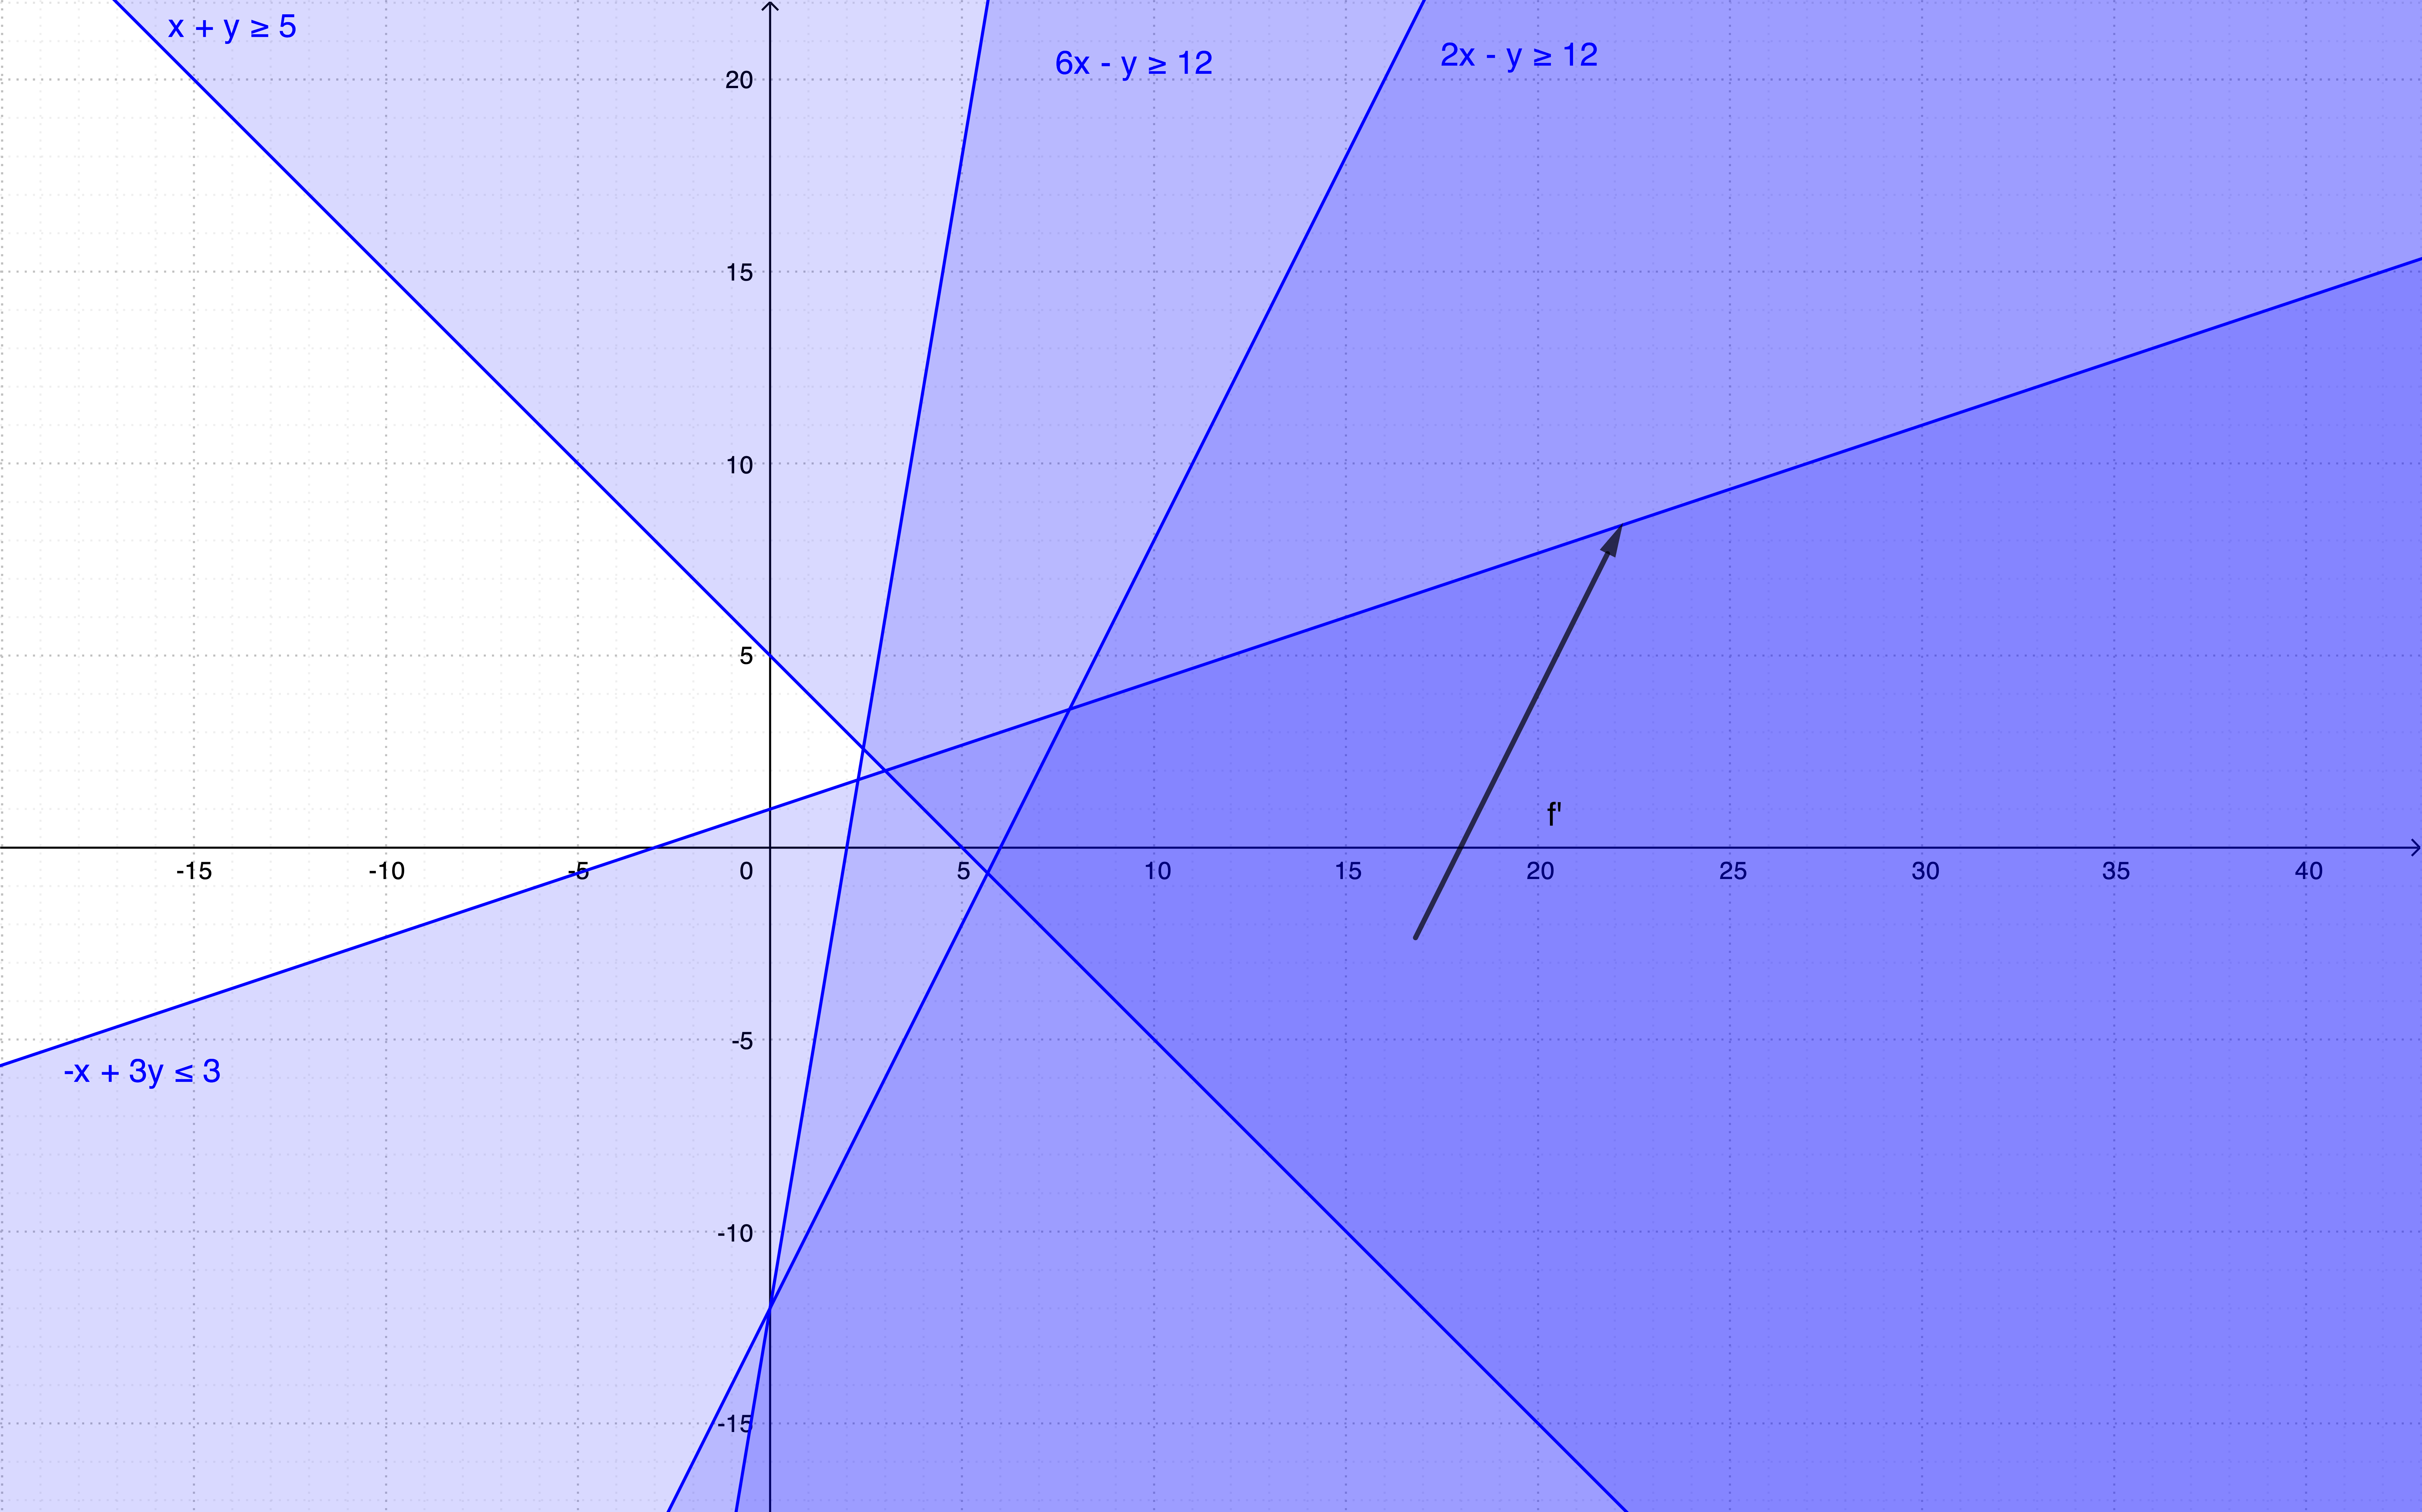
\includegraphics[width=\textwidth]{Plotii.png}
  \end{center}
\end{figure}
\end{proof}
\vspace{.15in}

\item[\textbf{(iii)}]\begin{align*}
  \text{Minimize:  }z = x - &2y\\
  \text{Subject to:  }x - 2y &\geq 4\\
  x + y &\leq 8\\
  x, y &\geq 0 
\end{align*}
\begin{proof}[Solution]
Plotting the first two inequality constraints we see that there feasible set is bounded. 
Finding our descent direction $-\nabla z = (-1, 2)^T$. Finally we see that our descent direction 
is pointing towards the $x - 2y \leq 4$ inequality so anywhere on the line $x - 2y = 4$ where we 
maintain feasible is a solution to this linear program.  

\begin{figure}[H]
\begin{center}
  \caption{First two inequality constraints with descent direction $f'$. (Plotted with GeoGebra)}
  \includegraphics[width=\textwidth]{Plotiii.png}
\end{center}
\end{figure}
\end{proof}
\vspace{.15in}



\item[\textbf{(iv)}]\begin{align*}
  \text{Minimize:  }z = -x - &y\\
  \text{Subject to:  }x - y &\geq 1\\
  x - 2y &\leq 2\\
  x, y &\geq 0 
\end{align*}
\begin{proof}[Solution]
Plotting the first two inequality constraints we see that there feasible set is bounded. 
Finding our descent direction $-\nabla z = (1, 1)^T$. Finally we see that our descent direction 
is pointing towards the $x - 2y \leq 2$ inequality and in a direction of unboundedness. Thus there is 
no minimum.

\begin{figure}[H]
\begin{center}
  \caption{First two inequality constraints with descent direction $f'$. (Plotted with GeoGebra)}
  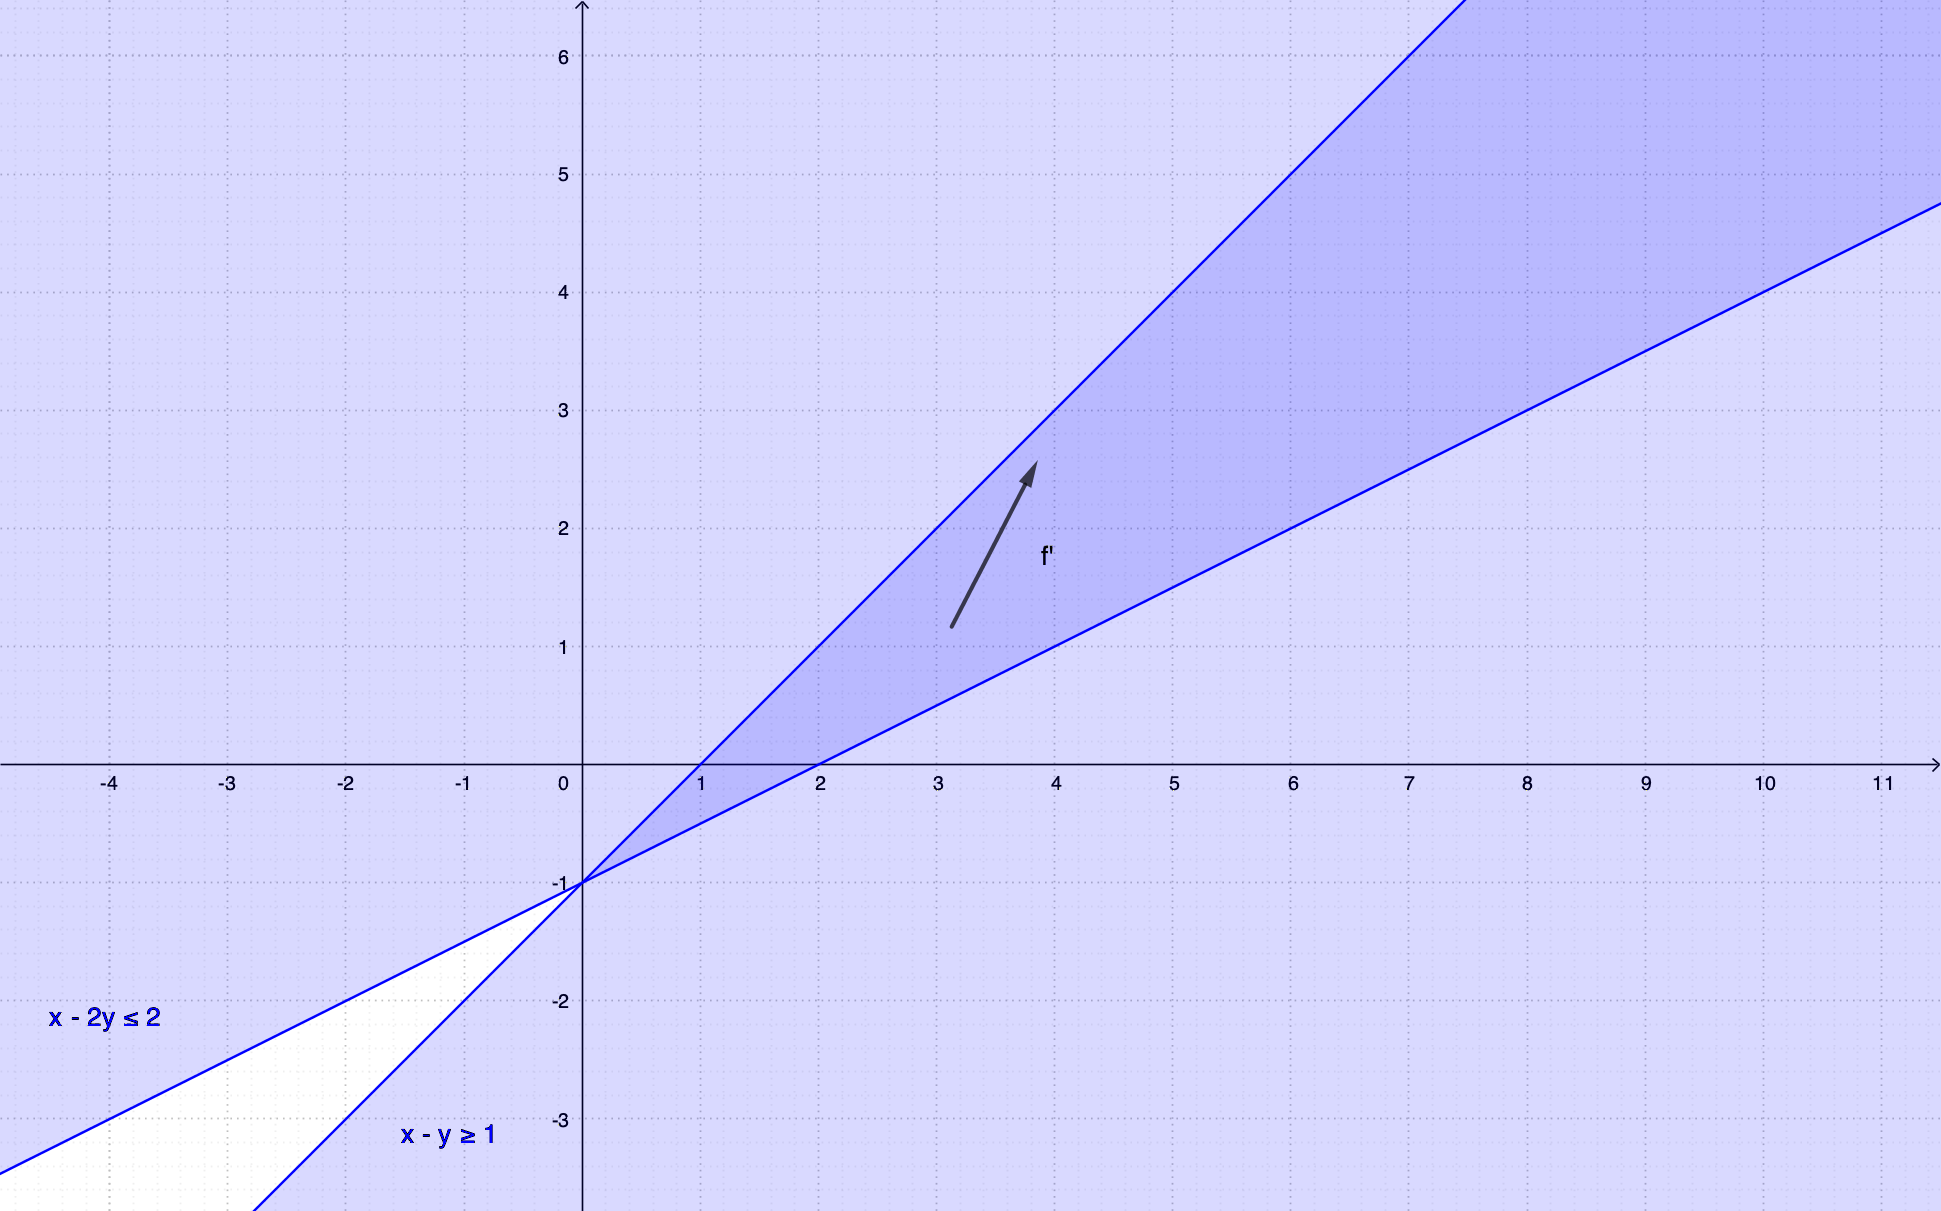
\includegraphics[width=\textwidth]{Plotiv.png}
\end{center}
\end{figure}
\end{proof}
\end{enumerate}
\end{exercise}
\vspace{.5in}


\begin{exercise}{1.2} Find graphically all the values of the parameter $a$ such that 
  $(-3, 4)^T$ is the optimal solution of the following problem:
  \begin{align*}
    \text{Maximize:  }z = ax + &(2 - a)y\\
    \text{Subject to:  }4x + 3y &\leq 0\\
    2x + 3y &\leq 7\\
    x + y &\leq 1 
  \end{align*}
  Looking at the plot of the feasible set, for $(-3, 4)^T$ to be the optimal solution our ascent 
  direction $\nabla z = (a, 2 - a)$ must be a convex combination of the two vectors orthogonal 
  to the inequalities that produce the intersection at $(-3, 4)^T$, namely $u = (1,1)^T$ and $v = (4, 3)^T$. 

  \begin{figure}[H]
    \begin{center}
      \caption{Plotting the feasible set with orthogonal vectors $u$ and $v$. (Plotted with GeoGebra)}
      \includegraphics[width=\textwidth]{Plotv.png}
    \end{center}
    \end{figure}
  Thus $(-3, 4)^T$ is an optimal solution for all $\nabla z$ where for all $0 \leq \alpha \leq 1$,
  \begin{equation*}
    \nabla z = 
    \begin{pmatrix}
      a\\
      2 - a
    \end{pmatrix}
     = 
     \alpha
     \begin{pmatrix}
      1\\
      1
    \end{pmatrix}
    + 
    (1 - \alpha)
    \begin{pmatrix}
      4\\
      3
    \end{pmatrix}.
  \end{equation*}
  Note that we didn't use strict inequalities for $\alpha$ since $(-3, 4)^T$ would still be an optimal solution in those cases, just not the only one. 
  
\end{exercise}








\end{document}


































